% В этом документе преамбула

%%% Работа с русским языком
\usepackage{cmap}					% поиск в PDF
\usepackage{mathtext} 				% русские буквы в формулах
\usepackage[T2A]{fontenc}			% кодировка
\usepackage[utf8]{inputenc}			% кодировка исходного текста
\usepackage[english,russian]{babel}	% локализация и переносы
\usepackage{indentfirst}			% чтобы первый абзац в разделе отбивался красной строкой
\frenchspacing						% тонкая настройка пробелов

%%% Приведение начертания букв и знаков к русской типографской традиции
\renewcommand{\epsilon}{\ensuremath{\varepsilon}}
\renewcommand{\phi}{\ensuremath{\varphi}}			% буквы "эпсилон"
\renewcommand{\kappa}{\ensuremath{\varkappa}}		% буквы "каппа"
\renewcommand{\le}{\ensuremath{\leqslant}}			% знак меньше или равно
\renewcommand{\leq}{\ensuremath{\leqslant}}			% знак меньше или равно
\renewcommand{\ge}{\ensuremath{\geqslant}}			% знак больше или равно
\renewcommand{\geq}{\ensuremath{\geqslant}}			% знак больше или равно
\renewcommand{\emptyset}{\varnothing}				% знак пустого множества

%%% Дополнительная работа с математикой
\usepackage{amsmath,amsfonts,amssymb,amsthm,mathtools} % AMS
\usepackage{icomma} % "Умная" запятая: $0,2$ --- число, $0, 2$ --- перечисление

%% Номера формул
\mathtoolsset{showonlyrefs=true} % Показывать номера только у тех формул, на которые есть \eqref{} в тексте.

%% Свои команды

% операции, не определённые (или имеющие иные обохначения) в мат. пакетах
\DeclareMathOperator{\sgn}{\mathop{sgn}}				% ф-ия sgn
\renewcommand{\tg}{\mathop{\mathrm{tg}}\nolimits}		% обозначение тангенса

%% Перенос знаков в формулах (по Львовскому)
\newcommand*{\hm}[1]{#1\nobreak\discretionary{}
{\hbox{$\mathsurround=0pt #1$}}{}}

%%% Работа с картинками
\usepackage{graphicx}  % Для вставки рисунков
\graphicspath{{images/}{images2/}}  % папки с картинками
\setlength\fboxsep{3pt} % Отступ рамки \fbox{} от рисунка
\setlength\fboxrule{1pt} % Толщина линий рамки \fbox{}
\usepackage{wrapfig} % Обтекание рисунков текстом

%%% Работа с таблицами
\usepackage{array,tabularx,tabulary,booktabs} % Дополнительная работа с таблицами
\usepackage{longtable}  % Длинные таблицы
\usepackage{multirow} % Слияние строк в таблице

%%% Теоремы
\theoremstyle{plain} % Это стиль по умолчанию, его можно не переопределять.
\newtheorem{theorem}{Теорема}[section]
\newtheorem{lemma}{Лемма}[section]
\newtheorem{definition}[theorem]{Определение}
\newtheorem{property}{Свойство}
 
\theoremstyle{definition} % "Определение"
\newtheorem{corollary}{Следствие}[theorem]
\newtheorem{exmp}{Пример}[section]
 
\theoremstyle{remark} % "Примечание"
\newtheorem*{nonum}{Решение}
\newtheorem*{evidence}{Доказательство}
\newtheorem*{remark}{Примечание}

%%% Программирование
\usepackage{etoolbox} % логические операторы

%%% Страница
\usepackage{extsizes} % Возможность сделать 14-й шрифт
\usepackage{geometry} % Простой способ задавать поля
	\geometry{top=25mm}
	\geometry{bottom=35mm}
	\geometry{left=35mm}
	\geometry{right=20mm}

%\usepackage{fancyhdr} % Колонтитулы
% 	\pagestyle{fancy}
 	%\renewcommand{\headrulewidth}{0pt}  % Толщина линейки, отчеркивающей верхний колонтитул
% 	\lfoot{Нижний левый}
% 	\rfoot{Нижний правый}
% 	\rhead{Верхний правый}
% 	\chead{Верхний в центре}
% 	\lhead{Верхний левый}
%	\cfoot{Нижний в центре} % По умолчанию здесь номер страницы

\usepackage{setspace} % Интерлиньяж (межстрочные интервалы)
%\onehalfspacing % Интерлиньяж 1.5
%\doublespacing % Интерлиньяж 2
%\singlespacing % Интерлиньяж 1

\usepackage{lastpage} % Узнать, сколько всего страниц в документе.

\usepackage{soulutf8} % Модификаторы начертания

\usepackage{hyperref}
\usepackage[usenames,dvipsnames,svgnames,table,rgb]{xcolor}
\hypersetup{				% Гиперссылки
    unicode=true,           % русские буквы в раздела PDF
    pdftitle={Заголовок},   % Заголовок
    pdfauthor={Автор},      % Автор
    pdfsubject={Тема},      % Тема
    pdfcreator={Создатель}, % Создатель
    pdfproducer={Производитель}, % Производитель
    pdfkeywords={keyword1} {key2} {key3}, % Ключевые слова
    colorlinks=true,       	% false: ссылки в рамках; true: цветные ссылки
    linkcolor=MidnightBlue,          % внутренние ссылки
    citecolor=black,        % на библиографию
    filecolor=magenta,      % на файлы
    urlcolor=blue           % на URL
}

\usepackage{csquotes} % Еще инструменты для ссылок

%\usepackage[style=authoryear,maxcitenames=2,backend=biber,sorting=nty]{biblatex}

\usepackage{multicol} % Несколько колонок

%%% Работа с графикой
\usepackage{tikz}
\usetikzlibrary{calc}
\usepackage{tkz-euclide}
\usetikzlibrary{arrows}
\usepackage{pgfplots}
\usepackage{pgfplotstable}

%%% Настройка подписей к плавающим объектам
\usepackage{floatrow}	% размещение
\usepackage{caption}	% начертание
\captionsetup[figure]{labelfont=bf,textfont=it,font=footnotesize}	% нумерация и надпись курсивом
% для подфигур: заголовок подписи полужирный, текст заголовка обычный
% выравнивание является неровным (т.е. выровненным по левому краю)
% singlelinecheck = off означает, что настройка выравнивания используется, даже если заголовок имеет длину только одну строку.
% если singlelinecheck = on, то заголовок всегда центрируется, когда заголовок состоит только из одной строки.
\captionsetup[subfigure]{labelfont=bf,textfont=normalfont,singlelinecheck=off,justification=raggedright}

%%% Stuff для графиков и рисунков



\title{Теория вероятностей и мат. статистика \\ ИДЗ2}
\date{18.04.2020}
\author{Почаев Никита Алексеевич, гр. 8381 \\ \href{mailto:pochaev.nik@gmail.com}{pochaev.nik@gmail.com} \\ Преподаватель: Малов Сергей Васильевич}

\begin{document}
	
\renewcommand{\figurename}{Рисунок}

\maketitle

\begin{figure}[H]
	\center{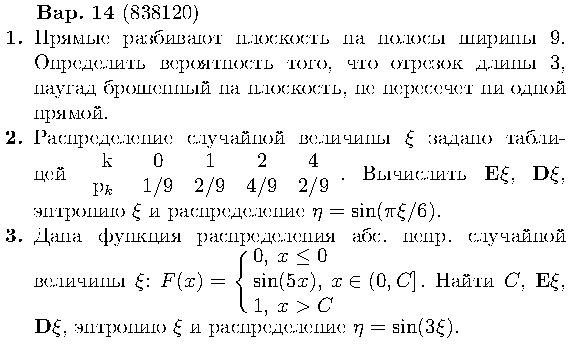
\includegraphics[scale=1]{./media/Задание.pdf}}
\end{figure}

\section*{Задача 1.}

Данная задача является переформулированной версией \textit{задачи Бюффона о бросании иглы}. Положим $l$ - длина иглы (отрезка), $t$ - расстояние между параллельными линиями (ширина полосы).

Пусть $x$ - расстояние от центра иглы (отрезка) до ближайшей параллельной линии, также положим $\theta$ как угол между иглой и одной из параллельных прямых.

Равномерная функции плотности распределения (ФПР) вероятности величины $x$ между 0 и $\frac{t}{2}$ имеет вид:
\[
\begin{cases}
	\frac{2}{t}, 0 \le x \le \frac{t}{2} \\
	0 - \text{ в остальных случаях}
\end{cases}
\]
Здесь $x=0$ представляет собой иглу, центр которой лежит ровно на прямой, а $x=\frac{t}{2}$ иглу, идеально центрированную между двумя линиями. Равномерная ФПР предполагает, что игла с одинаковой вероятностью упадёт в любом месте указанного диапазона, но не может выпасть за его пределы.
\begin{figure}[H]
	\center{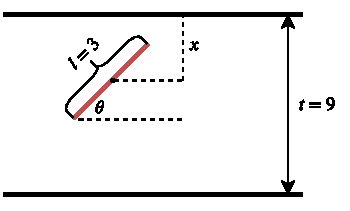
\includegraphics[scale=1.3]{./media/task_1_1.pdf}}
\end{figure}
Равномерная ФПР величины $\theta$ между 0 и $\frac{\pi}{2}$ имеет вид:
\[
\begin{cases}
	\frac{2}{\pi}, 0 \le \theta \le \frac{\pi}{2} \\
	0 - \text{ в остальных случаях}
\end{cases}
\]
Здесь $\theta=0$ радиан представляет собой иглу, расположенную параллельную отмеченным линиям, а $\theta = \frac{\pi}{2}$ радиан представляет иглу, расположенную перпендикулярно к отмеченным линиям. Любой угол в этом диапазоне считается одинаково вероятным результатом.

Две случайные величины $x$ и $\theta$ являются независимыми, следовательно, функций совместного распределения имеет вид:
\[
\begin{cases}
	\frac{4}{t \pi}, 0 \le x \le \frac{t}{2}, 0 \le \theta \le \frac{\pi}{2} \\
	0 - \text{ в остальных случаях}
\end{cases}
\]
Игла (отрезок) пересечёт линию, если $x \le \dfrac{l}{2} \sin \theta$.

В условиях данной задачи $l < t \Rightarrow$ интегрирование функции плотности совместной вероятности даёт вероятность того, что игла пересечет линию (обозначим данной событие за $A$):
\[
P(A) = \int_{\theta = 0}^{\frac{\pi}{2}} \int_{x=0}^{\frac{l}{2} \sin \theta} \frac{4}{t \pi} dx d \theta =
\int_{\theta = 0}^{\frac{\pi}{2}} \left[ \int_{x=0}^{\frac{l}{2} \sin \theta} \frac{4}{t \pi} dx \right] d \theta =
\int_{\theta = 0}^{\frac{\pi}{2}} \left[ \textcolor{Grey}{ \frac{4x}{\pi t} \bigg|_{x=0}^{\frac{1}{2} \sin \theta} = \frac{4(l \sin \theta)}{2 \pi t} - \frac{4 \times 0}{\pi t} = \frac{2l \sin \theta}{\pi t} } \right] d \theta =
\]
\[
= \left( - \frac{2l \cos \theta}{\pi t} \right) \bigg|_{\theta = 0}^{\frac{\pi}{2}} = \left( - \frac{2 l \cos \left(\frac{\pi}{2}\right)}{\pi t} \right) - \left( - \frac{2 l \cos (0)}{\pi t} \right) = \frac{2l}{\pi t}
\]

По условию задачи необходимо найти вероятность $P(\bar A)$ - отрезок не пересечёт прямую, что соотвествует обратному событию, т.е.:
\[
P(\bar A) = 1 - P(A) = 1 - \frac{2l}{\pi t} = 1 - \frac{2 \cdot 3}{9 \cdot \pi} \approx 0.787793409
\]

Графически решение данной задачи можно представить следующим образом:
\begin{figure}[H]
	\center{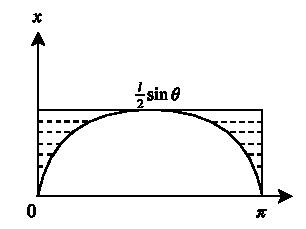
\includegraphics[scale=1.2]{./media/task_1_2.pdf}}
\end{figure}

\noindent\textbf{Ответ:} 0.787793409

\section*{Задача 2.}

Перепишем таблицу:
\begin{table}[H]
	\centering\makegapedcells
	\begin{tabular}{|c|c|c|c|c|}
		\hline
		$k$        & 0             & 1             & 2             & 4             \\ \hline
		$P(\xi=k)$ & $\frac{1}{9}$ & $\frac{2}{9}$ & $\frac{4}{9}$ & $\frac{2}{9}$ \\ \hline
	\end{tabular}
\end{table}
Величина дискретная $\Rightarrow$
\[
E\xi = \sum_{k} k \cdot P(\xi = k) = 0 \cdot \frac{1}{9} + 1 \cdot \frac{2}{9} + 2 \cdot \frac{4}{9} + 4 \cdot \frac{2}{9} = 2
\]
\[
E\xi^2 = 0^2 \cdot \frac{1}{9} + 1^2 \cdot \frac{2}{9} + 2^2 \cdot \frac{4}{9} + 4^2 \cdot \frac{2}{9} = \left(\frac{5 \sqrt{2}}{3}\right)^2 \approx 5.55556
\]
\[
D\xi = E(\xi - E\xi)^2 = E\xi^2 - (E\xi)^2 = \left(\frac{5 \sqrt{2}}{3}\right)^2 - 4 = \frac{14}{9} \approx 1.\bar{5}
\]

\[
\eta = \sin (\pi \frac{\xi}{6})
\]
\[
\xi = 0: \eta = 0; ~~~~~~~~~ \xi = 1: \eta = \frac{1}{2}; ~~~~~~~~~ \xi = 2: \eta = \frac{\sqrt{3}}{2}; ~~~~~~~~~ \xi = 4: \eta = \frac{\sqrt{3}}{2}
\]
Таким образом:
\[
\supp \xi = \{ 0, 1, 2, 4 \}
\]
\[
\supp \eta = \left\{ 0, \frac{1}{2}, \frac{\sqrt{3}}{2}, \frac{\sqrt{3}}{2} \right\}
\]
\[
p(\eta = 0) = \frac{1}{9} ~~~~~~~~~ p\left(\eta = \frac{1}{2}\right) = \frac{2}{9} ~~~~~~~~~ p\left(\eta = \frac{\sqrt{3}}{2}\right) = p(\{\xi = 2\} \cup \{\xi = 4\}) = \frac{4}{9} + \frac{2}{9} = \frac{2}{3}
\]
\begin{table}[H]
	\centering\makegapedcells
	\begin{tabular}{|c|c|c|c|}
		\hline
		$\eta$     & $0$           & $\frac{1}{2}$ & $\frac{\sqrt{3}}{2}$ \\ \hline
		$p_{\eta}$ & $\frac{1}{9}$ & $\frac{2}{9}$ & $\frac{2}{3}$        \\ \hline
	\end{tabular}
\end{table}
\[
F_{\eta} (x) =
\begin{cases}
0, &x \le 0 \\
\frac{1}{9}, &x \in (0, \frac{1}{2}] \\
\frac{1}{3}, &x \in (\frac{1}{2}, \frac{\sqrt{3}}{2}] \\
1, &x > \frac{\sqrt{3}}{2}
\end{cases}
\]

\section*{Задача 3.}

Плотность распределения случайной величины:
\[
p_{\xi} =
\begin{cases}
5 \cos (5x), &x \in (0, C] \\
0, &x \in (-\infty; 0] \cup (C; +\infty]
\end{cases}
\]
\[
\int_{-\infty}^{\infty} p_{\xi} (x) dx = 5 \int_{0}^{C} \cos (5x) dx = \sin (5x) \bigg|_{0}^{C} = \sin(5C) = 1 \Rightarrow 5C \ge \frac{\pi}{2} \Rightarrow C = \frac{\pi}{10} 
\]
Таким образом,
\[
p_{\xi}(x) =
\begin{cases}
5 \cos (5x), x \in [0, \frac{\pi}{10}] \\
0 - \text{ в остальных случаях}
\end{cases}
\]
$\xi$ - абсолютно непрерывная величина $\Rightarrow$
\[
E\xi = \int_{-\infty}^{\infty} x \cdot p_{\xi} (x) dx = \int_{0}^{\frac{\pi}{10}} x \cdot 5 \cos (5x) dx = 
x \sin (5x) \bigg|_{0}^{\frac{\pi}{10}} - \int_{0}^{\frac{\pi}{10}} \sin (5x) dx = 
\frac{\pi}{10} - \frac{\cos (5x)}{5} \bigg|_{0}^{\frac{\pi}{2}} = \frac{1}{10} (\pi - 2)
\]
Аналогично получаем:
\[
E\xi^2 = \int_{-\infty}^{\infty} x^2 \cdot p_{\xi} (x) dx = \int_{0}^{\frac{\pi}{10}} x^2 \cdot 5 \cos (5x) dx = \dots =
\frac{1}{100} (\pi^2 - 8)
\]

\[
D\xi = E(\xi - E\xi)^2 = E\xi^2 - (E\xi)^2 = \frac{1}{100} (\pi^2 - 8) - \left(\frac{1}{10} (\pi - 2)\right)^2 \approx 0.005663706
\]

\[
p\left(\xi \in \left[0, \frac{\pi}{10}\right]\right) = 1 \text{, т.е. } \supp \xi \in \left[0, \frac{\pi}{10}\right] \Rightarrow \supp(\eta) = \left[0, \frac{1}{4}(1+\sqrt{5})\right]
\]

\[
F_{\eta} = P(\eta < x) = p(\sin (3 \xi) < x) = p \left(\xi < \frac{1}{3} \arcsin x \right) = F_{\xi} \left(\frac{1}{3} \arcsin x\right) = \sin (3 \arcsin x)
\]

\[
F_{\eta}(x) =
\begin{cases}
0, &x < 0 \\
\sin (3 \arcsin x), &x \in \left[ 0, \frac{1}{4}(1+\sqrt{5}) \right] \\
1, &x > \frac{1}{4}(1+\sqrt{5})
\end{cases}
\]

\end{document} 